\scanpage{100}
\margin{$S\unsure{\sigma|\gamma}=(D\Delta\unsure{\sigma|\gamma}_K)(1)$}
\figure{\begin{tikzpicture}[x=1cm,y=1cm]
\draw[->](.7,0)..controls(-.6,0)and(-.5,.2)..(-.4,.7)..controls(-.4,1.1)and(.5,1.3)..(.8,1.6)..controls(1,1.9)and(.7,2.2)..(.3,2.6)..controls(-.1,3)and(.9,3.1)..(1.6,3.4);
\end{tikzpicture}}
\[
\underset{\sim}{\operatorname{Ext}}^i_{K/k}(G,S\underline{\unsure{\sigma|\gamma}})
\xrightarrow{\sim}
\underset{\sim}{\operatorname{Ext}}^{i\unsure{*}}_{k\text{-gr}}
(\Gamma^{\deleted{\unsure{*}}}G^*,\unsure{\sigma|\gamma})
\]
isom si $G$ \uline{affine} sans \unsure{composantes} $G_a$
\[
\underset{\sim}{\underline{\operatorname{Ext}}}^{i}_{K/k}(G,S\unsure{\sigma|\gamma})
\longrightarrow
\underset{\sim}{\underline{\operatorname{Ext}}}^{2i}(\Gamma G^*,\unsure{\sigma|\gamma})
\]
pour
\[
\underline{\operatorname{Ext}}^i_{K/k}(G,S\unsure{\sigma|\gamma})
\longrightarrow \underline{\operatorname{Ext}}^i
\]
\margin{\deleted{$\unsure{\Gamma}_{K/k}G$}\quad $R^*f_{K/k}$}

\noindent 1) $K$-\uline{groupes algébriques}.
\diagram{\begin{tikzcd}[column sep=large,row sep=small]
 & \text{nul pr }i>2\arrow[d,dash,bend right] & \\
\operatorname{Ext}\arrow[d,dash] &
\underline{\operatorname{Ext}}\arrow[d] & H^p\arrow[d]\\
\begin{gathered}\text{nature arithmétique}\\\text{ie ``globale''}\end{gathered} &
\begin{gathered}\text{nature}\\\text{géom.}\end{gathered} &
\begin{gathered}\text{nature arithmétique}\\\text{ie. ``globale''}\end{gathered}
\end{tikzcd}}
\uline{de $K$-groupes algébriques}

\noindent 2) \uline{Dualité de Cartier}. Extension aux
$\unsure{\mathcal K|\mathcal R}\operatorname{Gr}_K$

\margin{\figure{
\begin{tikzpicture}\draw (0,0)--(.4,.25);\draw (.02,-.04)--(.42,.21);\end{tikzpicture}}}
\noindent 3) \unsure{Quasi-groupes} algébriques, leurs
$\operatorname{Ext},\underline{\operatorname{Ext}},H^p$

\noindent 4) \uline{Dualité de Serre-\unsure{Pontrjagin}}

\noindent 5) Le foncteur $\underline\Gamma_{K/k}$
\inserted{de Néron-\unsure{Weil}}

\margin{\figure{
\begin{tikzpicture}\draw (0,0)--(.4,.25);\draw (.02,-.04)--(.42,.21);\end{tikzpicture}}}
\noindent 6) Les foncteurs \deleted{$\unsure{\Gamma}_{K/k}$}
\[
\underset{\sim}{\underline{\operatorname{Ext}}}^{*}_{K/k}(F,G),
\quad\underset{\sim}{\underline H}^{*}_{K/k}(G)
\]
\inserted{\[
E^*_{K/k}(F,G)\qquad E_{K/k}(G)
\]}
\margin{nul pr $i>3$}

\noindent 7) L'hom. fondamental.

\margin{\figure{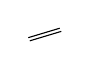
\begin{tikzpicture}\draw (0,0)--(.4,.12);\draw (.02,-.04)--(.42,.08);\end{tikzpicture}}}
\noindent 8) Le th. de dualité.
\mspage{99}

